\PassOptionsToPackage{unicode=true}{hyperref} % options for packages loaded elsewhere
\PassOptionsToPackage{hyphens}{url}
%
\documentclass[ignorenonframetext,]{beamer}
\usepackage{pgfpages}
\setbeamertemplate{caption}[numbered]
\setbeamertemplate{caption label separator}{: }
\setbeamercolor{caption name}{fg=normal text.fg}
\beamertemplatenavigationsymbolsempty
\usepackage{lmodern}
\usepackage{amssymb,amsmath}
\usepackage{ifxetex,ifluatex}
\usepackage{fixltx2e} % provides \textsubscript
\ifnum 0\ifxetex 1\fi\ifluatex 1\fi=0 % if pdftex
  \usepackage[T1]{fontenc}
  \usepackage[utf8]{inputenc}
  \usepackage{textcomp} % provides euro and other symbols
\else % if luatex or xelatex
  \usepackage{unicode-math}
  \defaultfontfeatures{Ligatures=TeX,Scale=MatchLowercase}
\fi
% use upquote if available, for straight quotes in verbatim environments
\IfFileExists{upquote.sty}{\usepackage{upquote}}{}
% use microtype if available
\IfFileExists{microtype.sty}{%
\usepackage[]{microtype}
\UseMicrotypeSet[protrusion]{basicmath} % disable protrusion for tt fonts
}{}
\IfFileExists{parskip.sty}{%
\usepackage{parskip}
}{% else
\setlength{\parindent}{0pt}
\setlength{\parskip}{6pt plus 2pt minus 1pt}
}
\usepackage{hyperref}
\hypersetup{
            pdftitle={Fitting spatial and spatiotemporal models},
            pdfauthor={Eric Ward},
            pdfborder={0 0 0},
            breaklinks=true}
\urlstyle{same}  % don't use monospace font for urls
\newif\ifbibliography
\usepackage{color}
\usepackage{fancyvrb}
\newcommand{\VerbBar}{|}
\newcommand{\VERB}{\Verb[commandchars=\\\{\}]}
\DefineVerbatimEnvironment{Highlighting}{Verbatim}{commandchars=\\\{\}}
% Add ',fontsize=\small' for more characters per line
\usepackage{framed}
\definecolor{shadecolor}{RGB}{248,248,248}
\newenvironment{Shaded}{\begin{snugshade}}{\end{snugshade}}
\newcommand{\AlertTok}[1]{\textcolor[rgb]{0.94,0.16,0.16}{#1}}
\newcommand{\AnnotationTok}[1]{\textcolor[rgb]{0.56,0.35,0.01}{\textbf{\textit{#1}}}}
\newcommand{\AttributeTok}[1]{\textcolor[rgb]{0.77,0.63,0.00}{#1}}
\newcommand{\BaseNTok}[1]{\textcolor[rgb]{0.00,0.00,0.81}{#1}}
\newcommand{\BuiltInTok}[1]{#1}
\newcommand{\CharTok}[1]{\textcolor[rgb]{0.31,0.60,0.02}{#1}}
\newcommand{\CommentTok}[1]{\textcolor[rgb]{0.56,0.35,0.01}{\textit{#1}}}
\newcommand{\CommentVarTok}[1]{\textcolor[rgb]{0.56,0.35,0.01}{\textbf{\textit{#1}}}}
\newcommand{\ConstantTok}[1]{\textcolor[rgb]{0.00,0.00,0.00}{#1}}
\newcommand{\ControlFlowTok}[1]{\textcolor[rgb]{0.13,0.29,0.53}{\textbf{#1}}}
\newcommand{\DataTypeTok}[1]{\textcolor[rgb]{0.13,0.29,0.53}{#1}}
\newcommand{\DecValTok}[1]{\textcolor[rgb]{0.00,0.00,0.81}{#1}}
\newcommand{\DocumentationTok}[1]{\textcolor[rgb]{0.56,0.35,0.01}{\textbf{\textit{#1}}}}
\newcommand{\ErrorTok}[1]{\textcolor[rgb]{0.64,0.00,0.00}{\textbf{#1}}}
\newcommand{\ExtensionTok}[1]{#1}
\newcommand{\FloatTok}[1]{\textcolor[rgb]{0.00,0.00,0.81}{#1}}
\newcommand{\FunctionTok}[1]{\textcolor[rgb]{0.00,0.00,0.00}{#1}}
\newcommand{\ImportTok}[1]{#1}
\newcommand{\InformationTok}[1]{\textcolor[rgb]{0.56,0.35,0.01}{\textbf{\textit{#1}}}}
\newcommand{\KeywordTok}[1]{\textcolor[rgb]{0.13,0.29,0.53}{\textbf{#1}}}
\newcommand{\NormalTok}[1]{#1}
\newcommand{\OperatorTok}[1]{\textcolor[rgb]{0.81,0.36,0.00}{\textbf{#1}}}
\newcommand{\OtherTok}[1]{\textcolor[rgb]{0.56,0.35,0.01}{#1}}
\newcommand{\PreprocessorTok}[1]{\textcolor[rgb]{0.56,0.35,0.01}{\textit{#1}}}
\newcommand{\RegionMarkerTok}[1]{#1}
\newcommand{\SpecialCharTok}[1]{\textcolor[rgb]{0.00,0.00,0.00}{#1}}
\newcommand{\SpecialStringTok}[1]{\textcolor[rgb]{0.31,0.60,0.02}{#1}}
\newcommand{\StringTok}[1]{\textcolor[rgb]{0.31,0.60,0.02}{#1}}
\newcommand{\VariableTok}[1]{\textcolor[rgb]{0.00,0.00,0.00}{#1}}
\newcommand{\VerbatimStringTok}[1]{\textcolor[rgb]{0.31,0.60,0.02}{#1}}
\newcommand{\WarningTok}[1]{\textcolor[rgb]{0.56,0.35,0.01}{\textbf{\textit{#1}}}}
% Prevent slide breaks in the middle of a paragraph:
\widowpenalties 1 10000
\raggedbottom
\setbeamertemplate{part page}{
\centering
\begin{beamercolorbox}[sep=16pt,center]{part title}
  \usebeamerfont{part title}\insertpart\par
\end{beamercolorbox}
}
\setbeamertemplate{section page}{
\centering
\begin{beamercolorbox}[sep=12pt,center]{part title}
  \usebeamerfont{section title}\insertsection\par
\end{beamercolorbox}
}
\setbeamertemplate{subsection page}{
\centering
\begin{beamercolorbox}[sep=8pt,center]{part title}
  \usebeamerfont{subsection title}\insertsubsection\par
\end{beamercolorbox}
}
\AtBeginPart{
  \frame{\partpage}
}
\AtBeginSection{
  \ifbibliography
  \else
    \frame{\sectionpage}
  \fi
}
\AtBeginSubsection{
  \frame{\subsectionpage}
}
\setlength{\emergencystretch}{3em}  % prevent overfull lines
\providecommand{\tightlist}{%
  \setlength{\itemsep}{0pt}\setlength{\parskip}{0pt}}
\setcounter{secnumdepth}{0}

% set default figure placement to htbp
\makeatletter
\def\fps@figure{htbp}
\makeatother


\title{Fitting spatial and spatiotemporal models}
\providecommand{\subtitle}[1]{}
\subtitle{FISH 507 -- Applied Time Series Analysis}
\author{Eric Ward}
\date{07 Feb 2019}

\begin{document}
\frame{\titlepage}

\begin{frame}{What we've learned so far}
\protect\hypertarget{what-weve-learned-so-far}{}

\begin{itemize}
\item
  Time series can be useful for identifying structure, improving
  precision, and accuracy of forecasts
\item
  Modeling multivariate time series

  \begin{itemize}
  \tightlist
  \item
    e.g.~MARSS() function, with each observed time series mapped to a
    single discrete state
  \end{itemize}
\item
  Using DFA

  \begin{itemize}
  \tightlist
  \item
    Structure determined by factor loadings
  \end{itemize}
\end{itemize}

\end{frame}

\begin{frame}{Response generally the same variable (not separate
species)}
\protect\hypertarget{response-generally-the-same-variable-not-separate-species}{}

\begin{itemize}
\tightlist
\item
  Making inference about population as a whole involves modeling pink as
  well as blue time series
\end{itemize}

\begin{center}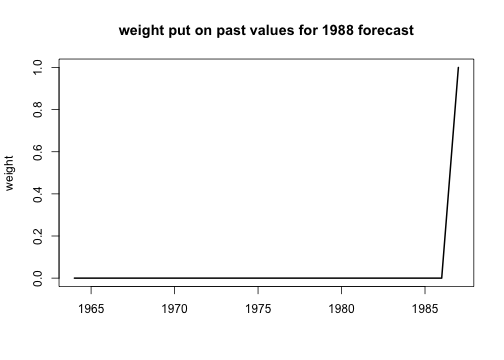
\includegraphics{lec_18_spatiotemporal_files/figure-beamer/unnamed-chunk-1-1} \end{center}

\end{frame}

\begin{frame}{Lots of time series -\textgreater{} complicated covariance
matrices}
\protect\hypertarget{lots-of-time-series---complicated-covariance-matrices}{}

\begin{itemize}
\item
  Last week, in talking about Gaussian process models, we showed the
  number of covariance matrix parameters = \(m*(m+1)/2\)

  \begin{itemize}
  \tightlist
  \item
    problematic for \textgreater{} 5 or so time series
  \end{itemize}
\item
  MARSS solutions: diagonal matrices or `equalvarcov'
\item
  DFA runs into same issues with estimating unconstrained \(R\) matrix
\end{itemize}

\end{frame}

\begin{frame}{Potential problems with both the MARSS and DFA approach}
\protect\hypertarget{potential-problems-with-both-the-marss-and-dfa-approach}{}

\begin{itemize}
\item
  Sites separated by large distances may be grouped together
\item
  Sites close to one another may be found to have very different
  dynamics
\end{itemize}

\end{frame}

\begin{frame}{Are there biological mechanisms that may explain this?}
\protect\hypertarget{are-there-biological-mechanisms-that-may-explain-this}{}

\begin{itemize}
\tightlist
\item
  Puget Sound Chinook salmon

  \begin{itemize}
  \tightlist
  \item
    21 populations generally cluster into 2-3 groups based on genetics
  \item
    Historically large hatchery programs
  \end{itemize}
\item
  Hood canal harbor seals

  \begin{itemize}
  \tightlist
  \item
    Visited by killer whales
  \end{itemize}
\end{itemize}

\begin{center}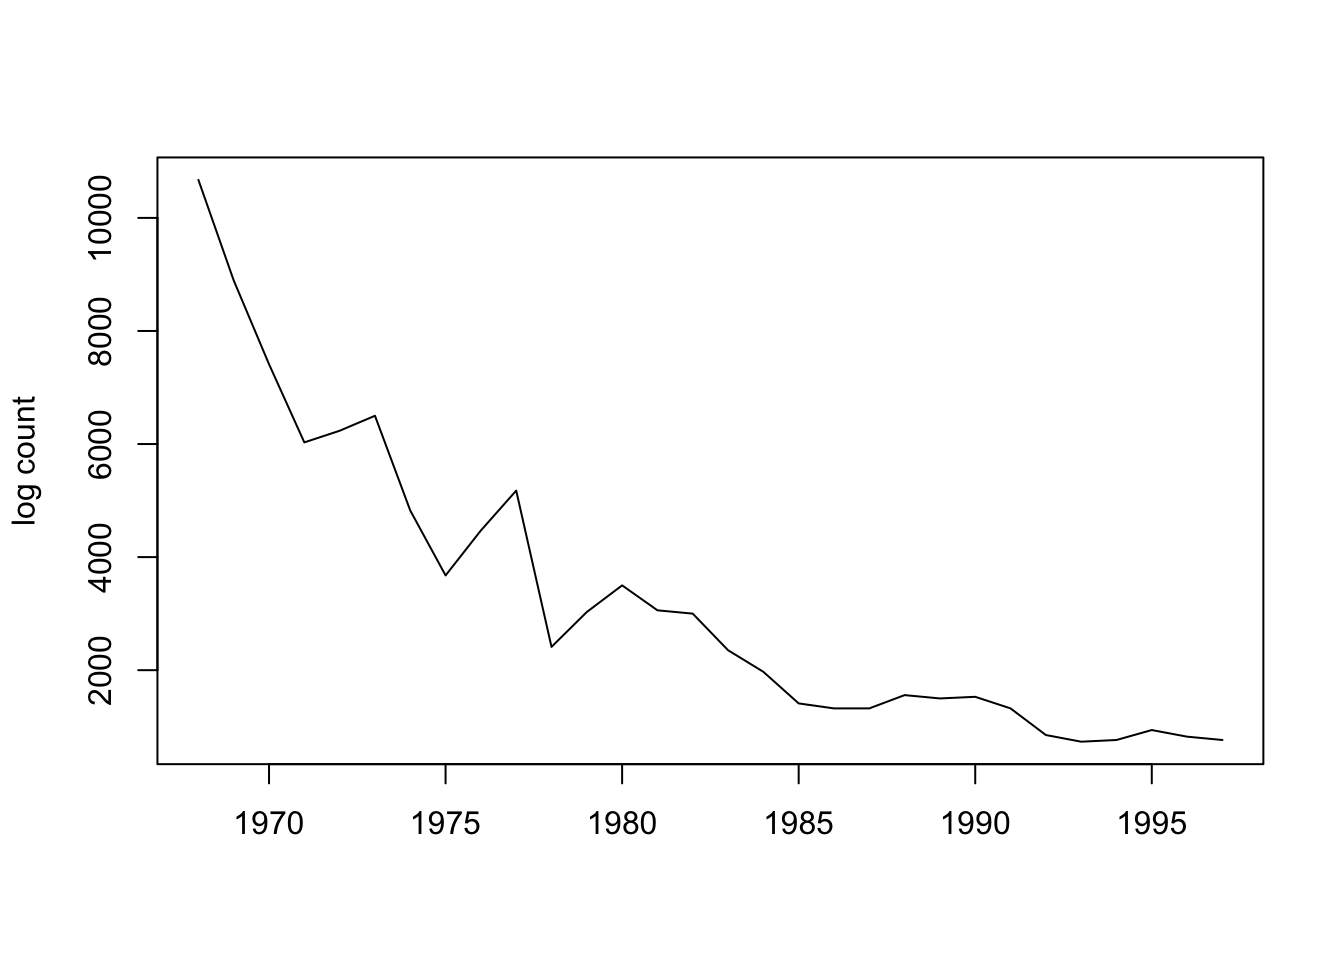
\includegraphics{lec_18_spatiotemporal_files/figure-beamer/unnamed-chunk-2-1} \end{center}

\end{frame}

\begin{frame}{Motivation of explicitly including spatial structure}
\protect\hypertarget{motivation-of-explicitly-including-spatial-structure}{}

\begin{itemize}
\item
  Adjacent sites can be allowed to covary
\item
  Estimated parameters greatly reduced to 2-5
\end{itemize}

\end{frame}

\begin{frame}{Types of spatial data}
\protect\hypertarget{types-of-spatial-data}{}

Point referenced data (aka geostatistical)

\begin{itemize}
\tightlist
\item
  Typically 2-D, but could be 1-D or 3-D (depth, altitude)
\item
  May be fixed station or random (e.g.~trawl surveys)
\end{itemize}

Point pattern data

\begin{itemize}
\tightlist
\item
  Spatially referenced based on outcomes (e.g.~presence)
\item
  Inference focused on describing clustering (or not)
\end{itemize}

Areal data

\begin{itemize}
\tightlist
\item
  Locations occur in blocks
\item
  counties, management zones, etc.
\end{itemize}

\end{frame}

\begin{frame}{Computationally convenient approaches}
\protect\hypertarget{computationally-convenient-approaches}{}

CAR (conditionally autoregressive models)

\begin{itemize}
\tightlist
\item
  Better suited for Bayesian methods
\item
  Goal of both is to write the distribution of a single prediction
  analytically in terms of the joint (y1, y2)
\end{itemize}

SAR (simultaneous autregressive models)

\begin{itemize}
\tightlist
\item
  Better suited for ML methods
\item
  Simultaneously model distribution of predicted values
\end{itemize}

`Autoregressive' in the sense of spatial dependency / correlation
between locations

\end{frame}

\begin{frame}{CAR models (Besag 1991)}
\protect\hypertarget{car-models-besag-1991}{}

\[{ Y }_{ i }=B{ X }_{ i }+{ \phi  }_{ i }i+{ \varepsilon  }_{ i }\]

\({ X }_{ i }\) are predictors (regression) \({ \phi }_{ i }i\) spatial
component, (aka markov random field) \({ \varepsilon }_{ i }\) residual
error term

\begin{itemize}
\tightlist
\item
  Create spatial adjacency matrix W, based on neighbors, e.g.
\item
  W(i,j) = 1 if neighbors, 0 otherwise
\item
  W often row-normalized (rows sum to 1)
\end{itemize}

\end{frame}

\begin{frame}{Adjacency matrix example}
\protect\hypertarget{adjacency-matrix-example}{}

\end{frame}

\begin{frame}{CAR models}
\protect\hypertarget{car-models}{}

In matrix form,

\[{ y\sim N\left( 0,{ \left( I-\rho W \right)  }^{ -1 }\widetilde { D }  \right) \\ { \widetilde { D }  }_{ ii }={ \sigma  }_{ i } }\]

\begin{itemize}
\tightlist
\item
  Implemented in `spdep', `CARBayes', etc
\end{itemize}

\end{frame}

\begin{frame}{SAR models}
\protect\hypertarget{sar-models}{}

\begin{itemize}
\tightlist
\item
  Simultaneous autoregressive model
\end{itemize}

\[{ y\sim N\left( 0,{ \left( I-\rho W \right)  }^{ -1 }\widetilde { D } { \left( I-\rho W \right)  }^{ -1 } \right) \\ { \widetilde { D }  }_{ ii }={ \sigma  }_{ i } }\]

\begin{itemize}
\tightlist
\item
  Remember that the CAR was
\end{itemize}

\[{ y\sim N\left( 0,{ \left( I-\rho W \right)  }^{ -1 }\widetilde { D }  \right) \\ { \widetilde { D }  }_{ ii }={ \sigma  }_{ i } }\]

\end{frame}

\begin{frame}{Commonalities of both approaches}
\protect\hypertarget{commonalities-of-both-approaches}{}

\begin{itemize}
\item
  Adjacency matrix W can also instead be modified to include distance
\item
  Models spatial dependency as a function of single parameter \(\rho\)
\item
  Models don't include time dimension in spatial field

  \begin{itemize}
  \tightlist
  \item
    One field estimated for all time steps
  \end{itemize}
\end{itemize}

\end{frame}

\begin{frame}{Problems with these approaches}
\protect\hypertarget{problems-with-these-approaches}{}

Wall (2004) ``A close look at the spatial structure implied by the CAR
and SAR models''.

\begin{itemize}
\tightlist
\item
  Note: not a 1-to-1 mapping of distance and correlation
\end{itemize}

\end{frame}

\begin{frame}{Alternative to CAR \& SAR}
\protect\hypertarget{alternative-to-car-sar}{}

\begin{itemize}
\tightlist
\item
  model elements of Q as functions
\item
  Create matrix D, as pairwise distances
\item
  This can be 1-D, or any dimension

  \begin{itemize}
  \tightlist
  \item
    We'll use Euclidian distances for 2-D
  \end{itemize}
\end{itemize}

\end{frame}

\begin{frame}{Squared exponential covariance}
\protect\hypertarget{squared-exponential-covariance}{}

\end{frame}

\begin{frame}{Squared exponential covariance}
\protect\hypertarget{squared-exponential-covariance-1}{}

\end{frame}

\begin{frame}{Squared exponential covariance}
\protect\hypertarget{squared-exponential-covariance-2}{}

\end{frame}

\begin{frame}{Considerations for time series models}
\protect\hypertarget{considerations-for-time-series-models}{}

Should spatial dependency be included? If so, how to model it?

\begin{itemize}
\tightlist
\item
  Constant
\item
  Time varying
\item
  Autoregressive
\item
  Random walk
\item
  Independent variation
\end{itemize}

\end{frame}

\begin{frame}{Model-based geostatistical approaches}
\protect\hypertarget{model-based-geostatistical-approaches}{}

\begin{enumerate}
\item
  Generalized least squares
\item
  Bayesian methods in spBayes, glmmfields
\item
  INLA models
\item
  Spatial GAMs
\item
  VAST (TMB)
\end{enumerate}

\end{frame}

\begin{frame}{Method 1: using gls()}
\protect\hypertarget{method-1-using-gls}{}

Generalized least squares function - similar syntax to lm, glm, etc.

Flexible correlation structures - corExp() - corGaus() - corLin() -
corSpher()

Allows irregularly spaced data / NAs - unlike Arima(), auto.arima(),
etc.

\end{frame}

\begin{frame}{WA Snotel sites}
\protect\hypertarget{wa-snotel-sites}{}

\end{frame}

\begin{frame}{Modeling WA Snotel data}
\protect\hypertarget{modeling-wa-snotel-data}{}

We'll use Snow Water Equivalent (SWE) data in Washington state

70 SNOTEL sites

\begin{itemize}
\tightlist
\item
  we'll focus only on Cascades
\end{itemize}

1981-2013

Initially start using just the February SWE data

1518 data points (only 29 missing values!)

\end{frame}

\begin{frame}[fragile]{Use AIC to evaluate different correlation models}
\protect\hypertarget{use-aic-to-evaluate-different-correlation-models}{}

\begin{Shaded}
\begin{Highlighting}[]
\NormalTok{mod.exp =}\StringTok{ }\KeywordTok{gls}\NormalTok{(Feb }\OperatorTok{~}\StringTok{ }\NormalTok{elev, }
  \DataTypeTok{correlation =} \KeywordTok{corExp}\NormalTok{(}\DataTypeTok{form=}\OperatorTok{~}\NormalTok{lat}\OperatorTok{+}\NormalTok{lon,}\DataTypeTok{nugget=}\NormalTok{T), }
  \DataTypeTok{data =}\NormalTok{ y[}\KeywordTok{which}\NormalTok{(}\KeywordTok{is.na}\NormalTok{(y}\OperatorTok{$}\NormalTok{Feb)}\OperatorTok{==}\NormalTok{F }\OperatorTok{&}\StringTok{ }\NormalTok{y}\OperatorTok{$}\NormalTok{Water.Year}\OperatorTok{==}\DecValTok{2013}\NormalTok{),])}
\KeywordTok{AIC}\NormalTok{(mod.exp) =}\StringTok{ }\FloatTok{431.097}

\NormalTok{mod.gaus =}\StringTok{ }\KeywordTok{gls}\NormalTok{(Feb }\OperatorTok{~}\StringTok{ }\NormalTok{elev, }
  \DataTypeTok{correlation =} \KeywordTok{corGaus}\NormalTok{(}\DataTypeTok{form=}\OperatorTok{~}\NormalTok{lat}\OperatorTok{+}\NormalTok{lon,}\DataTypeTok{nugget=}\NormalTok{T), }
  \DataTypeTok{data =}\NormalTok{ y[}\KeywordTok{which}\NormalTok{(}\KeywordTok{is.na}\NormalTok{(y}\OperatorTok{$}\NormalTok{Feb)}\OperatorTok{==}\NormalTok{F }\OperatorTok{&}\StringTok{ }\NormalTok{y}\OperatorTok{$}\NormalTok{Water.Year}\OperatorTok{==}\DecValTok{2013}\NormalTok{),])}
\KeywordTok{AIC}\NormalTok{(mod.gaus) =}\StringTok{ }\FloatTok{433.485}
\end{Highlighting}
\end{Shaded}

\end{frame}

\begin{frame}[fragile]{Diagnostics: fitting variograms}
\protect\hypertarget{diagnostics-fitting-variograms}{}

\begin{Shaded}
\begin{Highlighting}[]
\NormalTok{var.exp <-}\StringTok{ }\KeywordTok{Variogram}\NormalTok{(mod.exp, }\DataTypeTok{form =}\OperatorTok{~}\StringTok{ }\NormalTok{lat}\OperatorTok{+}\NormalTok{lon)}
\KeywordTok{plot}\NormalTok{(var.exp,}\DataTypeTok{main=}\StringTok{"Exponential"}\NormalTok{,}\DataTypeTok{ylim=}\KeywordTok{c}\NormalTok{(}\DecValTok{0}\NormalTok{,}\DecValTok{1}\NormalTok{))}

\NormalTok{var.gaus <-}\StringTok{ }\KeywordTok{Variogram}\NormalTok{(mod.gaus, }\DataTypeTok{form =}\OperatorTok{~}\StringTok{ }\NormalTok{lat}\OperatorTok{+}\NormalTok{lon)}
\KeywordTok{plot}\NormalTok{(var.gaus,}\DataTypeTok{main=}\StringTok{"Gaussian"}\NormalTok{,}\DataTypeTok{ylim=}\KeywordTok{c}\NormalTok{(}\DecValTok{0}\NormalTok{,}\DecValTok{1}\NormalTok{))}
\end{Highlighting}
\end{Shaded}

\end{frame}

\begin{frame}{Exponential variogram}
\protect\hypertarget{exponential-variogram}{}

Semivariance = \(0.5 \quad Var({x}_{1},{x}_{2})\)\\
Semivariance = Sill - \(Cov({x}_{1},{x}_{2})\)

\end{frame}

\begin{frame}{Gaussian variogram}
\protect\hypertarget{gaussian-variogram}{}

\end{frame}

\begin{frame}{Extensions of these models}
\protect\hypertarget{extensions-of-these-models}{}

corExp and corGaus spatial structure useful for wide variety of models /
R packages

Linear/non-linear mixed effect models

\begin{itemize}
\tightlist
\item
  lme() / nlme() in nlme package
\end{itemize}

Generalized linear mixed models

\begin{itemize}
\tightlist
\item
  glmmPQL() in MASS package
\end{itemize}

Generalized additive mixed models

\begin{itemize}
\tightlist
\item
  gamm() in mgcv package
\end{itemize}

\end{frame}

\begin{frame}{Method 2: GAMs}
\protect\hypertarget{method-2-gams}{}

Previous approaches modeled errors as correlated

\begin{itemize}
\tightlist
\item
  Spatial GAMs generally model mean as spatially correlated
\end{itemize}

\end{frame}

\begin{frame}[fragile]{Example with SNOTEL data}
\protect\hypertarget{example-with-snotel-data}{}

First a simple GAM, with latitude and longtide.

\begin{itemize}
\tightlist
\item
  Note we're not transforming to UTM, but probably should
\item
  Note we're not including tensor smooths te(), but probably should
\end{itemize}

\begin{Shaded}
\begin{Highlighting}[]
\NormalTok{d =}\StringTok{ }\NormalTok{dplyr}\OperatorTok{::}\KeywordTok{filter}\NormalTok{(d, }\OperatorTok{!}\KeywordTok{is.na}\NormalTok{(Water.Year), }\OperatorTok{!}\KeywordTok{is.na}\NormalTok{(Feb)) }
\NormalTok{mod =}\StringTok{ }\KeywordTok{gam}\NormalTok{(Feb }\OperatorTok{~}\StringTok{ }\KeywordTok{s}\NormalTok{(Water.Year) }\OperatorTok{+}\StringTok{ }
\StringTok{    }\KeywordTok{s}\NormalTok{(Longitude, Latitude), }\DataTypeTok{data=}\NormalTok{d)}
\NormalTok{d}\OperatorTok{$}\NormalTok{resid =}\StringTok{ }\KeywordTok{resid}\NormalTok{(mod)}
\end{Highlighting}
\end{Shaded}

\end{frame}

\begin{frame}{Ok, let's look at the residuals}
\protect\hypertarget{ok-lets-look-at-the-residuals}{}

First, residuals through time

\begin{center}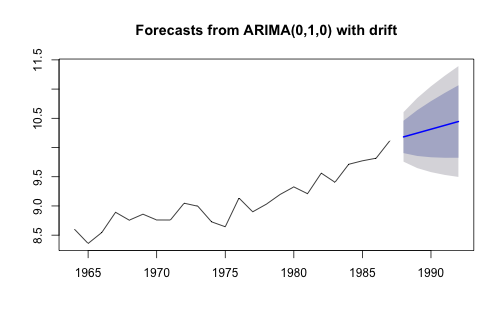
\includegraphics{lec_18_spatiotemporal_files/figure-beamer/unnamed-chunk-8-1} \end{center}

\end{frame}

\begin{frame}{Now residuals spatially}
\protect\hypertarget{now-residuals-spatially}{}

We'll use a subset of years here

\begin{center}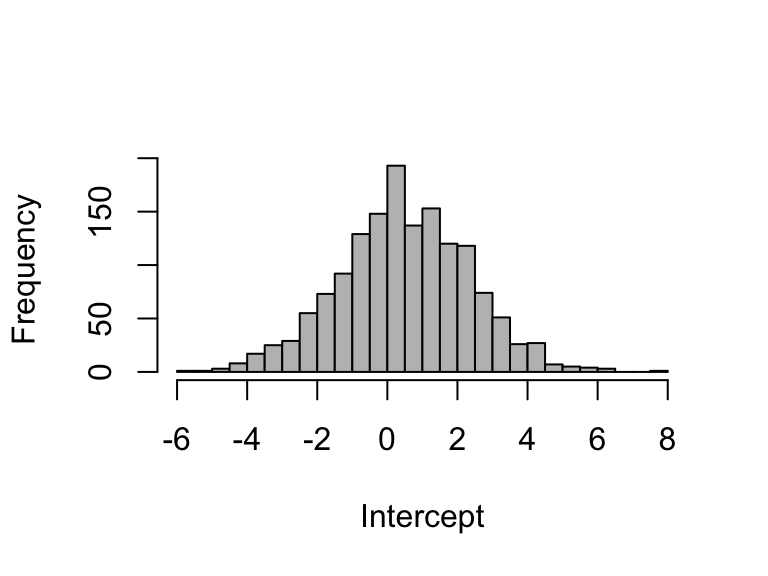
\includegraphics{lec_18_spatiotemporal_files/figure-beamer/unnamed-chunk-9-1} \end{center}

\end{frame}

\begin{frame}[fragile]{Two ways to include spatial temporal
interactions}
\protect\hypertarget{two-ways-to-include-spatial-temporal-interactions}{}

\begin{itemize}
\tightlist
\item
  What do these interactions mean in the context of our SNOTEL data?
\end{itemize}

\begin{enumerate}
\tightlist
\item
  First, spatial field may vary by year
\end{enumerate}

\begin{Shaded}
\begin{Highlighting}[]
\NormalTok{mod2 =}\StringTok{ }\KeywordTok{gam}\NormalTok{(Feb }\OperatorTok{~}\StringTok{ }\KeywordTok{s}\NormalTok{(Water.Year) }\OperatorTok{+}\StringTok{ }
\StringTok{    }\KeywordTok{s}\NormalTok{(Longitude, Latitude, }\DataTypeTok{by=}\KeywordTok{as.factor}\NormalTok{(Water.Year)), }\DataTypeTok{data=}\NormalTok{d)}
\NormalTok{d}\OperatorTok{$}\NormalTok{resid =}\StringTok{ }\KeywordTok{resid}\NormalTok{(mod2)}
\end{Highlighting}
\end{Shaded}

\end{frame}

\begin{frame}[fragile]{Two ways to include spatial temporal
interactions}
\protect\hypertarget{two-ways-to-include-spatial-temporal-interactions-1}{}

\begin{enumerate}
\setcounter{enumi}{1}
\tightlist
\item
  Spatial effect may be continuous and we can include space-time
  interaction
\end{enumerate}

\begin{itemize}
\tightlist
\item
  Why ti() instead of te() ? ti() only is the interaction where te()
  includes the main effects
\end{itemize}

\begin{Shaded}
\begin{Highlighting}[]
\NormalTok{mod2 =}\StringTok{ }\KeywordTok{gam}\NormalTok{(Feb }\OperatorTok{~}\StringTok{ }\KeywordTok{s}\NormalTok{(Longitude, Latitude) }\OperatorTok{+}\StringTok{ }\KeywordTok{s}\NormalTok{(Water.Year) }\OperatorTok{+}\StringTok{ }
\StringTok{    }\KeywordTok{ti}\NormalTok{(Longitude, Latitude,Water.Year, }\DataTypeTok{d=}\KeywordTok{c}\NormalTok{(}\DecValTok{2}\NormalTok{,}\DecValTok{1}\NormalTok{)), }\DataTypeTok{data=}\NormalTok{d)}
\NormalTok{d}\OperatorTok{$}\NormalTok{resid =}\StringTok{ }\KeywordTok{resid}\NormalTok{(mod2)}
\end{Highlighting}
\end{Shaded}

\end{frame}

\begin{frame}{GAM extensions and resources}
\protect\hypertarget{gam-extensions-and-resources}{}

Quickly evolving features for spatio-temporal models

\begin{itemize}
\tightlist
\item
  Random effects (gamm)
\item
  Interface with inla (g-inla)
\item
  Bayesian estimation (bam)
\end{itemize}

Lots of detailed examples and resources

*e.g.~ESA workshop by Simpson/Pederson/Ross/Miller

\url{https://noamross.github.io/mgcv-esa-workshop/}

\end{frame}

\begin{frame}{Potential limitations of spatial GAMs}
\protect\hypertarget{potential-limitations-of-spatial-gams}{}

\begin{itemize}
\item
  Hard to specify covariance structure explicitly
\item
  Hard to add constraints, like making spatial field be an AR(1) process
\item
  Motivates more custom approaches
\end{itemize}

\end{frame}

\begin{frame}{Bayesian: spBayes}
\protect\hypertarget{bayesian-spbayes}{}

Slightly more complicated syntax:

Specify:

\begin{itemize}
\tightlist
\item
  Priors on parameters
\item
  Tuning parameters for Metropolis sampling (jumping variance)
\item
  Starting / initial values
\item
  Covariance structure (``exponential'', ``gaussian'', ``matern'', etc)
\item
  Number of MCMC iterations / burn-in, etc.
\end{itemize}

\end{frame}

\begin{frame}[fragile]{Example with SNOTEL data}
\protect\hypertarget{example-with-snotel-data-1}{}

\begin{Shaded}
\begin{Highlighting}[]
\CommentTok{# This syntax is dependent on model parameters. See vignette}
\NormalTok{priors <-}\StringTok{ }\KeywordTok{list}\NormalTok{(}\StringTok{"beta.Norm"}\NormalTok{=}\KeywordTok{list}\NormalTok{(}\KeywordTok{rep}\NormalTok{(}\DecValTok{0}\NormalTok{,p), }
  \KeywordTok{diag}\NormalTok{(}\DecValTok{1000}\NormalTok{,p)), }\StringTok{"phi.Unif"}\NormalTok{=}\KeywordTok{c}\NormalTok{(}\DecValTok{3}\OperatorTok{/}\DecValTok{1}\NormalTok{, }\DecValTok{3}\OperatorTok{/}\FloatTok{0.1}\NormalTok{), }
  \StringTok{"sigma.sq.IG"}\NormalTok{=}\KeywordTok{c}\NormalTok{(}\DecValTok{2}\NormalTok{, }\DecValTok{2}\NormalTok{), }\StringTok{"tau.sq.IG"}\NormalTok{=}\KeywordTok{c}\NormalTok{(}\DecValTok{2}\NormalTok{, }\FloatTok{0.1}\NormalTok{))}

\CommentTok{# Phi is spatial scale parameter, sigma.sq is spatial variance, }
\CommentTok{# tau.sq = residual}
\NormalTok{starting <-}\StringTok{ }\KeywordTok{list}\NormalTok{(}\StringTok{"phi"}\NormalTok{=}\DecValTok{3}\OperatorTok{/}\FloatTok{0.5}\NormalTok{, }\StringTok{"sigma.sq"}\NormalTok{=}\DecValTok{50}\NormalTok{, }\StringTok{"tau.sq"}\NormalTok{=}\DecValTok{1}\NormalTok{)}

\CommentTok{# variance of normal proposals for Metropolis algorithm}
\NormalTok{tuning <-}\StringTok{ }\KeywordTok{list}\NormalTok{(}\StringTok{"phi"}\NormalTok{=}\FloatTok{0.1}\NormalTok{, }\StringTok{"sigma.sq"}\NormalTok{=}\FloatTok{0.1}\NormalTok{, }\StringTok{"tau.sq"}\NormalTok{=}\FloatTok{0.1}\NormalTok{)}

\NormalTok{m}\FloatTok{.1}\NormalTok{ <-}\StringTok{ }\KeywordTok{spLM}\NormalTok{(y}\OperatorTok{~}\NormalTok{X}\DecValTok{-1}\NormalTok{, }\DataTypeTok{coords=}\NormalTok{cords, }
  \DataTypeTok{n.samples=}\DecValTok{10000}\NormalTok{, }
  \DataTypeTok{cov.model =} \StringTok{"exponential"}\NormalTok{, }\DataTypeTok{priors=}\NormalTok{priors, }
  \DataTypeTok{tuning=}\NormalTok{tuning, }\DataTypeTok{starting=}\NormalTok{starting)}
\end{Highlighting}
\end{Shaded}

\end{frame}

\begin{frame}[fragile]{Coefficients need to be extracted}
\protect\hypertarget{coefficients-need-to-be-extracted}{}

\begin{Shaded}
\begin{Highlighting}[]
\NormalTok{##recover beta and spatial random effects}
\NormalTok{burn.in <-}\StringTok{ }\DecValTok{5000}
\NormalTok{m}\FloatTok{.1}\NormalTok{ <-}\StringTok{ }\KeywordTok{spRecover}\NormalTok{(m}\FloatTok{.1}\NormalTok{, }\DataTypeTok{start=}\NormalTok{burn.in, }\DataTypeTok{verbose=}\OtherTok{FALSE}\NormalTok{)}
\end{Highlighting}
\end{Shaded}

\end{frame}

\begin{frame}{Standard MCMC diagnostics}
\protect\hypertarget{standard-mcmc-diagnostics}{}

Output is of class `mcmc'

\end{frame}

\begin{frame}{Method 3: glmmfields}
\protect\hypertarget{method-3-glmmfields}{}

\begin{itemize}
\item
  New R package that implements these models using Stan
\item
  Easy to use formula syntax like gam() or spBayes()
\item
  Allows spatial field to be modeled with Multivariate-T field, as
  alternative to Multivariate-Normal to better capture extremes
\item
  Also includes lots of non-normal responses for observation model
\end{itemize}

\end{frame}

\begin{frame}[fragile]{glmmfields}
\protect\hypertarget{glmmfields}{}

Let's start with a simple model. This includes only 6 knots (probably
way too few) and 100 iterations (too few!) for run time.

\begin{itemize}
\tightlist
\item
  Time set to NULL here to fit a model with constant spatial field
\end{itemize}

\begin{Shaded}
\begin{Highlighting}[]
\NormalTok{m <-}\StringTok{ }\KeywordTok{glmmfields}\NormalTok{(Feb }\OperatorTok{~}\StringTok{ }\DecValTok{0}\NormalTok{, }\DataTypeTok{time =} \OtherTok{NULL}\NormalTok{,}
 \DataTypeTok{lat =} \StringTok{"Latitude"}\NormalTok{, }\DataTypeTok{lon =} \StringTok{"Longitude"}\NormalTok{, }\DataTypeTok{data =}\NormalTok{ d,}
 \DataTypeTok{nknots =} \DecValTok{6}\NormalTok{, }\DataTypeTok{iter =} \DecValTok{100}\NormalTok{, }\DataTypeTok{chains =} \DecValTok{2}\NormalTok{, }\DataTypeTok{seed =} \DecValTok{1}\NormalTok{)}
\end{Highlighting}
\end{Shaded}

\end{frame}

\begin{frame}[fragile]{glmmfields}
\protect\hypertarget{glmmfields-1}{}

Ok, now let's change the covariance function to matern, and estimate
separate spatial fields by year.

\begin{itemize}
\tightlist
\item
  The `estimate\_ar' argument is important for determining whether the
  field is an AR(1) process or independent by year
\end{itemize}

\begin{Shaded}
\begin{Highlighting}[]
\NormalTok{m <-}\StringTok{ }\KeywordTok{glmmfields}\NormalTok{(Feb }\OperatorTok{~}\StringTok{ }\DecValTok{0}\NormalTok{, }\DataTypeTok{time =} \StringTok{"Water.Year"}\NormalTok{,}
 \DataTypeTok{lat =} \StringTok{"Latitude"}\NormalTok{, }\DataTypeTok{lon =} \StringTok{"Longitude"}\NormalTok{, }\DataTypeTok{covariance=}\StringTok{"matern"}\NormalTok{,}
  \DataTypeTok{data =}\NormalTok{ d, }\DataTypeTok{nknots =} \DecValTok{6}\NormalTok{, }\DataTypeTok{iter =} \DecValTok{100}\NormalTok{, }\DataTypeTok{chains =} \DecValTok{2}\NormalTok{, }\DataTypeTok{seed =} \DecValTok{1}\NormalTok{,}
  \DataTypeTok{estimate_AR=}\OtherTok{FALSE}\NormalTok{)}
\end{Highlighting}
\end{Shaded}

\end{frame}

\begin{frame}[fragile]{glmmfields}
\protect\hypertarget{glmmfields-2}{}

Finally let's include an example with modeling the spatial field as a
Multivariate-t distribution

\begin{itemize}
\tightlist
\item
  We do this with the `estimate\_df' argument
\end{itemize}

\begin{Shaded}
\begin{Highlighting}[]
\NormalTok{m <-}\StringTok{ }\KeywordTok{glmmfields}\NormalTok{(Feb }\OperatorTok{~}\StringTok{ }\DecValTok{0}\NormalTok{, }\DataTypeTok{time =} \StringTok{"Water.Year"}\NormalTok{,}
 \DataTypeTok{lat =} \StringTok{"Latitude"}\NormalTok{, }\DataTypeTok{lon =} \StringTok{"Longitude"}\NormalTok{, }\DataTypeTok{covariance=}\StringTok{"matern"}\NormalTok{,}
  \DataTypeTok{data =}\NormalTok{ d, }\DataTypeTok{nknots =} \DecValTok{6}\NormalTok{, }\DataTypeTok{iter =} \DecValTok{100}\NormalTok{, }\DataTypeTok{chains =} \DecValTok{2}\NormalTok{, }\DataTypeTok{seed =} \DecValTok{1}\NormalTok{,}
  \DataTypeTok{estimate_AR=}\OtherTok{FALSE}\NormalTok{, }\DataTypeTok{estimate_df=} \OtherTok{TRUE}\NormalTok{)}
\end{Highlighting}
\end{Shaded}

\end{frame}

\begin{frame}{Method 4: INLA}
\protect\hypertarget{method-4-inla}{}

GP spatial models are extremely powerful

\begin{itemize}
\item
  May get overwhelmed by number of points
\item
  Approaches to incorporate knots using sparse covariance matrices
\item
  Integrated Nested Laplace Approximation
\item
  install.packages(``INLA'')
\end{itemize}

\end{frame}

\begin{frame}{Motivation of INLA}
\protect\hypertarget{motivation-of-inla}{}

Some problems contain simple spatial structure e.g.~the harbor seal data
in MARSS() with only 5 -- 7 time series

Others are much more complex

\begin{itemize}
\tightlist
\item
  WA SWE data
\item
  Fisheries survey data (1000s of points)
\end{itemize}

Including time-varying spatial fields becomes very computationally
difficult

Doing all of the above in a Bayesian setting can be prohibitive, but we
can use Laplace approximation

\end{frame}

\begin{frame}{Varying spatial fields example: eulachon-shrimp bycatch}
\protect\hypertarget{varying-spatial-fields-example-eulachon-shrimp-bycatch}{}

\end{frame}

\begin{frame}{INLA's approximation: SNOTEL data}
\protect\hypertarget{inlas-approximation-snotel-data}{}

How many points fall on vertices? Is the boundary area large enough?
Choosing this must be done very carefully!

\end{frame}

\begin{frame}{Estimation done via maximum likelihood}
\protect\hypertarget{estimation-done-via-maximum-likelihood}{}

\begin{itemize}
\tightlist
\item
  Estimates seems similar to those from gls() and spBayes()
\item
  Year included as numeric here (not significant)
\item
  Alternatively, we can include year in spatial field
\item
  Year can also be included as factor
\end{itemize}

\end{frame}

\begin{frame}{Projecting INLA estimates to surface}
\protect\hypertarget{projecting-inla-estimates-to-surface}{}

\end{frame}

\begin{frame}{Spatial SWE fields by year}
\protect\hypertarget{spatial-swe-fields-by-year}{}

\end{frame}

\begin{frame}[fragile]{Modeling intervention effects with spatial
models}
\protect\hypertarget{modeling-intervention-effects-with-spatial-models}{}

How do we model change points / break points in the mean in regression,
ARIMA models, or GAMs?

\begin{Shaded}
\begin{Highlighting}[]
\KeywordTok{lm}\NormalTok{(Feb }\OperatorTok{~}\StringTok{ }\NormalTok{Water.Year)}
\KeywordTok{gam}\NormalTok{(Feb }\OperatorTok{~}\StringTok{ }\KeywordTok{s}\NormalTok{(Water.Year))}
\KeywordTok{auto.arima}\NormalTok{(Feb, }\DataTypeTok{xreg=}\NormalTok{Water.Year)}
\end{Highlighting}
\end{Shaded}

\end{frame}

\begin{frame}[fragile]{Modeling intervention effects with spatial
models}
\protect\hypertarget{modeling-intervention-effects-with-spatial-models-1}{}

How do we model change points / break points in the mean in regression,
ARIMA models, or GAMs?

\begin{Shaded}
\begin{Highlighting}[]
\KeywordTok{lm}\NormalTok{(Feb }\OperatorTok{~}\StringTok{ }\NormalTok{Water.Year)}
\KeywordTok{gam}\NormalTok{(Feb }\OperatorTok{~}\StringTok{ }\KeywordTok{s}\NormalTok{(Water.Year))}
\KeywordTok{auto.arima}\NormalTok{(Feb, }\DataTypeTok{xreg=}\NormalTok{Water.Year)}
\end{Highlighting}
\end{Shaded}

\begin{itemize}
\tightlist
\item
  Use indicator functions before / after breakpoint
\end{itemize}

\end{frame}

\begin{frame}{Example: modeling spatiotemporal responses of fish to oil
spills}
\protect\hypertarget{example-modeling-spatiotemporal-responses-of-fish-to-oil-spills}{}

\href{https://link.springer.com/article/10.1007\%2Fs10661-018-6912-z}{Ward
et al.~2018}

2 approaches for looking at effects:

\begin{itemize}
\item
  indicator / change point associated with the spill
\item
  Or post-hoc approach to look at changes in spatial variability
  post-spill

  \begin{itemize}
  \tightlist
  \item
    why: lagged effects, non-stationary spatial effects
  \end{itemize}
\end{itemize}

\end{frame}

\begin{frame}{Example: modeling spatiotemporal responses of fish to oil
spills}
\protect\hypertarget{example-modeling-spatiotemporal-responses-of-fish-to-oil-spills-1}{}

\end{frame}

\begin{frame}{Example: modeling spatiotemporal responses of fish to oil
spills}
\protect\hypertarget{example-modeling-spatiotemporal-responses-of-fish-to-oil-spills-2}{}

\end{frame}

\end{document}
